\documentclass[tikz,border=3mm]{standalone}
\usepackage{amsmath}

\usetikzlibrary{matrix,positioning,fit,backgrounds,intersections}
\usetikzlibrary{calc}



\begin{document}

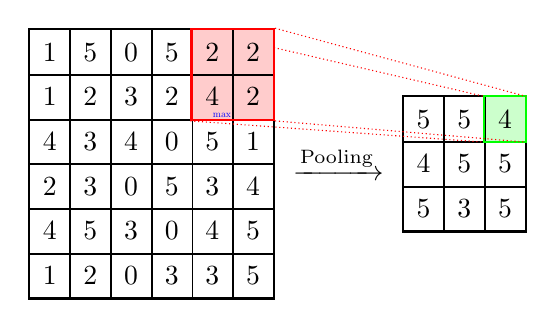
\begin{tikzpicture}[mmat/.style={matrix of math nodes,column sep=-\pgflinewidth/2,
   row sep=-\pgflinewidth/2,cells={nodes={draw,inner sep=5pt,ultra thin}},draw=#1,thick,inner sep=0pt},
   mmat/.default=black,
   node distance=0.3em]
 \matrix[mmat](mat1){
         1 & 5 & 0 & 5 & 2 & 2 \\ 
         1 & 2 & 3 & 2 & 4 & 2 \\ 
         4 & 3 & 4 & 0 & 5 & 1 \\ 
         2 & 3 & 0 & 5 & 3 & 4 \\ 
         4 & 5 & 3 & 0 & 4 & 5 \\ 
         1 & 2 & 0 & 3 & 3 & 5 \\
         };

\path (mat1-2-5.south east) node[anchor=south east,blue,scale=0.35,inner sep=2.2pt]{max};

      
 \node[fit=(mat1-1-5)(mat1-2-6),inner sep=0pt,draw,red,thick,name path=fit](f1){};
 \node[right=of mat1] (mul) {$\xrightarrow{\text{Pooling}}$};
 \matrix[mmat,right=of mul,name path=mat2](mat2){    
     5 & 5 & 4 \\ 
     4 & 5 & 5 \\ 
     5 & 3 & 5 \\ };
 \node[fit=(mat2-1-3)(mat2-1-3),inner sep=0pt,draw,green,thick,name path=pool](p1){};%%%
 \foreach \Anchor in {south west,north west,south east,north east}
 {\path[name path=test] (f1.\Anchor) -- (mat2-1-3.\Anchor);
 \draw[red,densely dotted,name intersections={of=test and fit,total=\t}]
 \ifnum\t>0 (intersection-\t) -- (mat2-1-3.\Anchor) \else
  (f1.\Anchor) -- (mat2-1-3.\Anchor)\fi;
}


\begin{scope}[on background layer]
    \fill[red!20] (f1.north west) rectangle (f1.south east);
\end{scope}
\begin{scope}[on background layer]
    \fill[green!20] (p1.north west) rectangle (p1.south east);
\end{scope}
\end{tikzpicture}
\end{document}